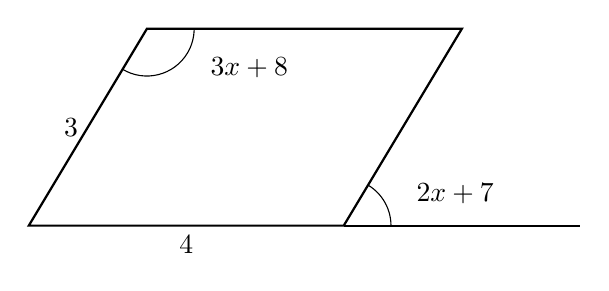
\begin{tikzpicture}[scale=1]

    % Define the vertices of the parallelogram
    \coordinate (A) at (0,0);
    \coordinate (B) at (4,0);
    \coordinate (C) at (5.5,2.5);
    \coordinate (D) at (1.5,2.5);

    % Draw the main parallelogram
    \draw[thick] (A) -- (B) -- (C) -- (D) -- cycle;

    % Draw the extended line to the right of the base (horizontal line)
    \draw[thick] (B) -- (7,0);

    % --- ARC FOR 3x + 8 (Top Left Corner) ---
    % Centered at D (1.5, 2.5)
    % Sweeps from the bottom-left side (DA) to the top side (DC)
    \draw (1.5,2.5) ++(239:0.6) arc (239:360:0.6);
    
    % --- ARC FOR 2x + 7 (Bottom Right Exterior) ---
    % Centered at B (4, 0)
    \draw (4,0) ++(0:0.6) arc (0:59:0.6);

    % Place the labels and measurements
    % Left side label
    \node[left] at (0.75, 1.25) {3};
    
    % Bottom side label
    \node[below] at (2, 0) {4};
    
    % --- SHIFTED 3x + 8 LABEL ---
    % Moved right to approximately (2.8, 2.0)
    \node at (2.8, 2.0) {$3x + 8$};
    
    % Exterior angle label
    \node[right] at (4.8, 0.4) {$2x + 7$};

\end{tikzpicture}